\begin{frame}{Single Shot Object Detection}
\begin{figure}
\centering
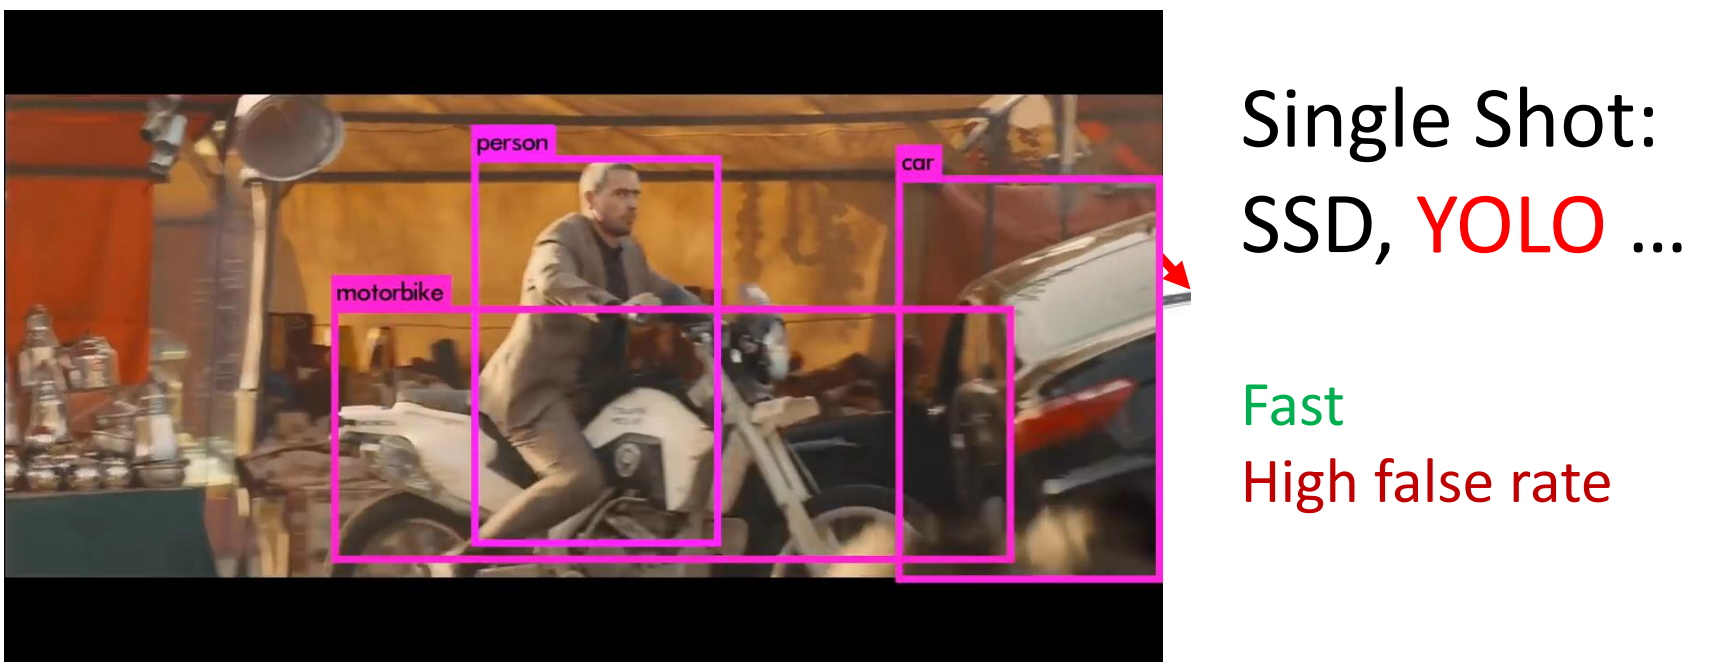
\includegraphics[width=1.0\textwidth,height=1.0\textheight,keepaspectratio]{images/obj-det/yolo_1.png}
\end{figure}
    
\end{frame}

\begin{frame}{YOLO - Overview}
\only<1>{
\begin{figure}
\centering
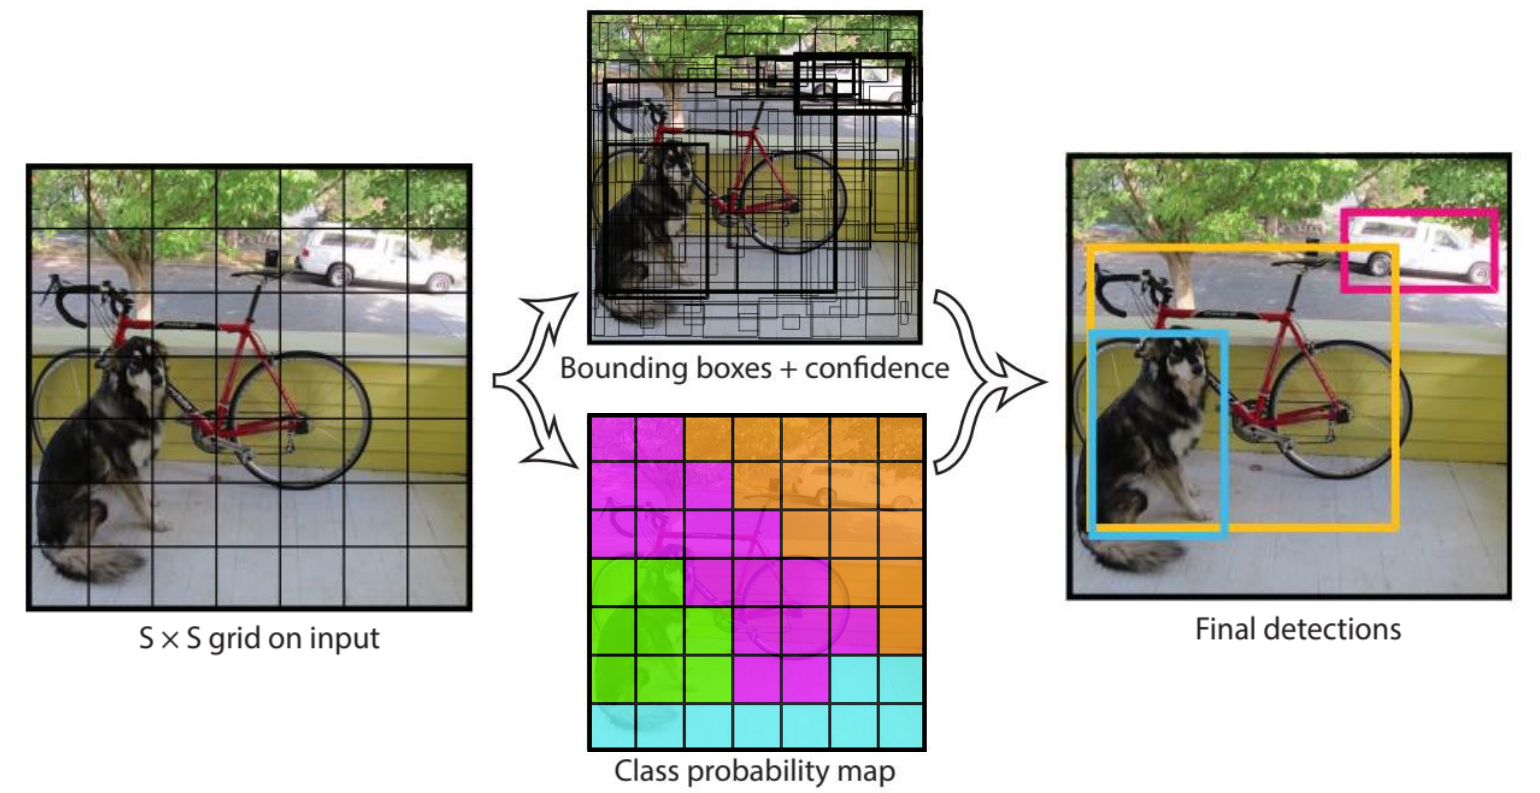
\includegraphics[width=1.0\textwidth,height=1.0\textheight,keepaspectratio]{images/obj-det/yolo_2.png}
\end{figure}
}

\only<2>{
\begin{figure}
\centering
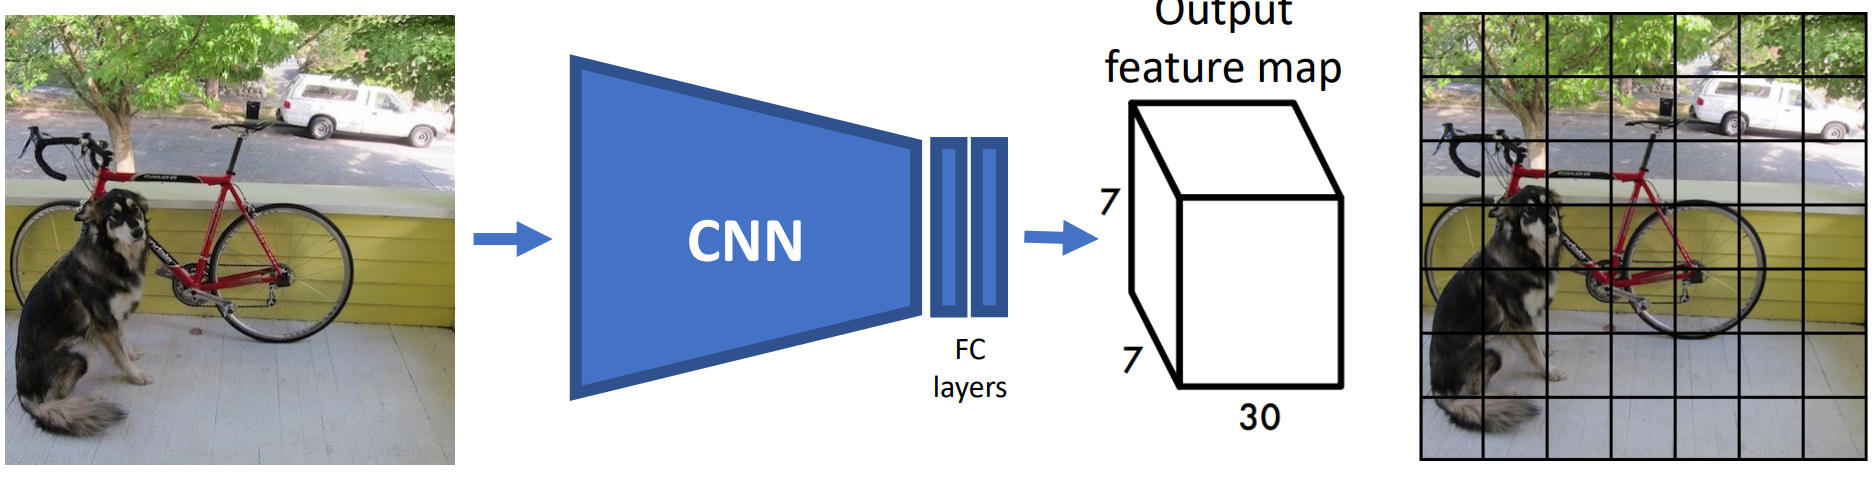
\includegraphics[width=1.0\textwidth,height=1.0\textheight,keepaspectratio]{images/obj-det/yolo_3.png}
\end{figure}
}
\only<3>{
\begin{figure}
\centering
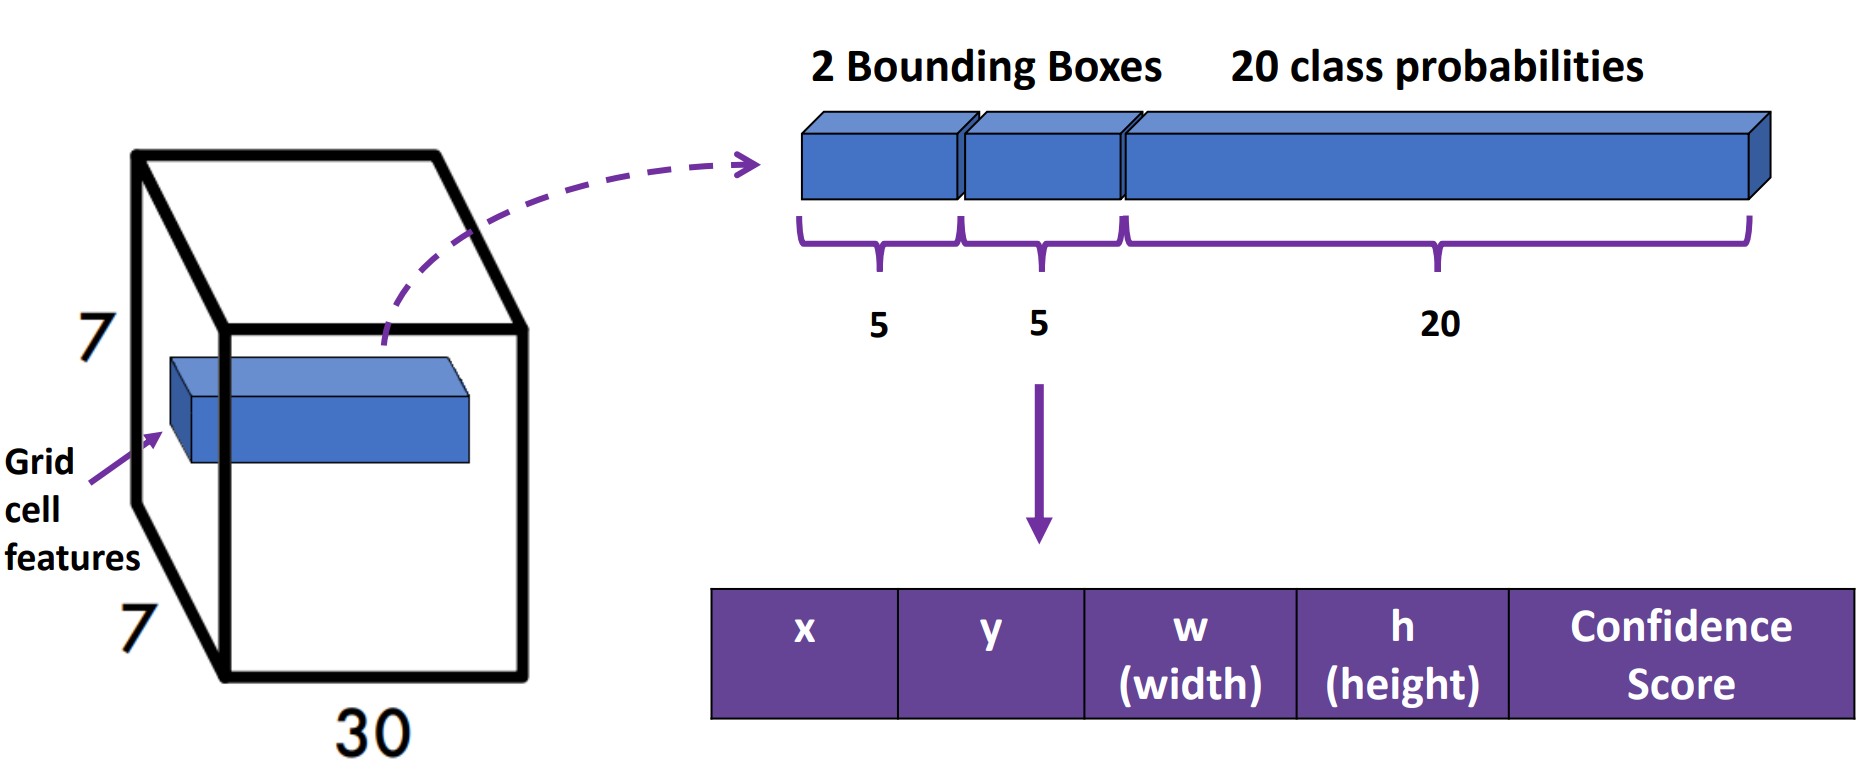
\includegraphics[width=1.0\textwidth,height=1.0\textheight,keepaspectratio]{images/obj-det/yolo_4.png}
\end{figure}
}
    
\end{frame}

\begin{frame}{YOLO}
\begin{columns}
    \begin{column}{0.5\textwidth}
    \onslide<2->{Each cell predicts}
    \begin{itemize}
        \item<3-> $B=2$ bounding boxes $(x,y,w,h) + $ confidence score
        \item<4-> $C=20$ class probabilities
        \vspace{1cm}
        \item<8-> Apply Non-Maximum Suppression
    \end{itemize}
    \end{column}
    
    \begin{column}{0.5\textwidth}
    \only<-2>{
    \begin{figure}
    \centering
    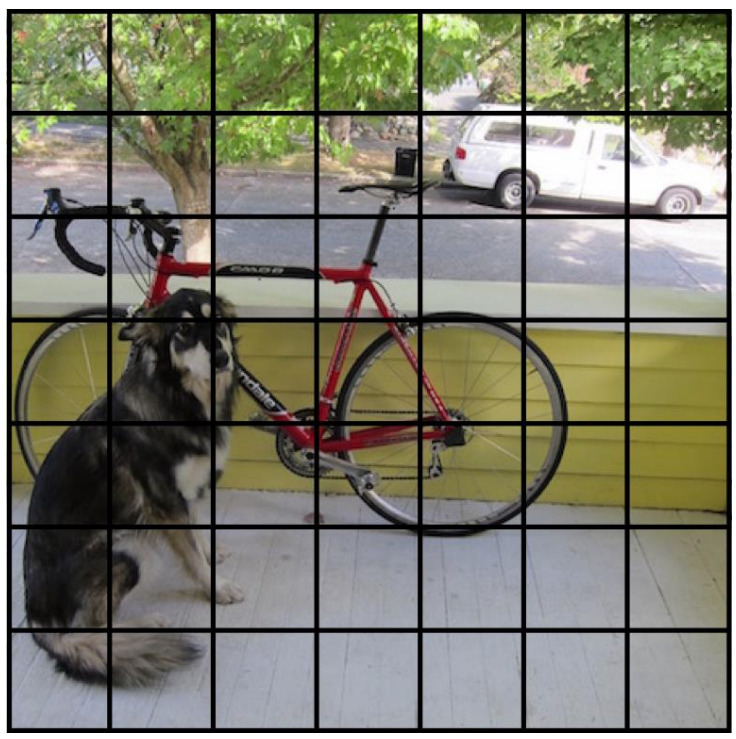
\includegraphics[width=1.0\textwidth,height=1.0\textheight,keepaspectratio]{images/obj-det/yolo_5.png}
    \end{figure}
    }

    \only<3-4>{
    \begin{figure}
    \centering
    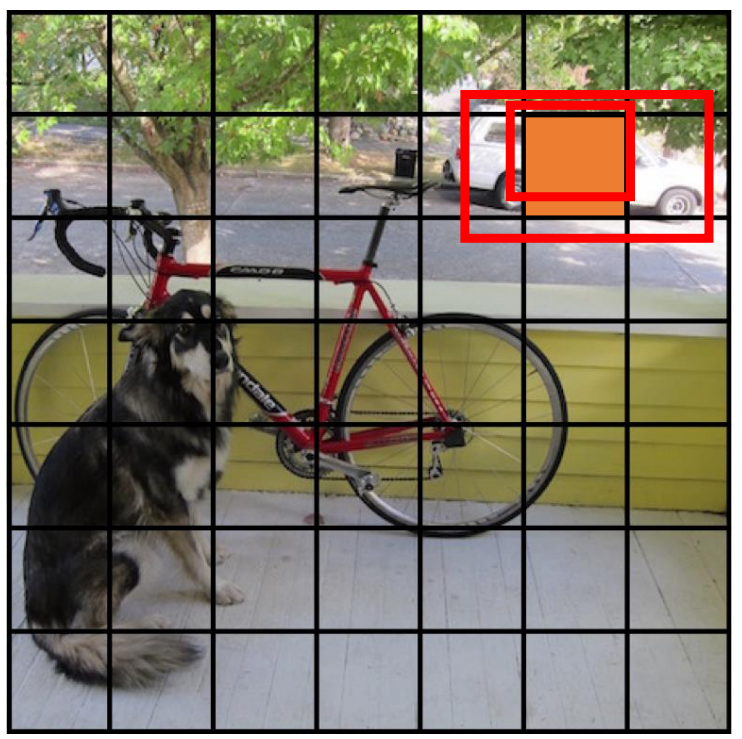
\includegraphics[width=1.0\textwidth,height=1.0\textheight,keepaspectratio]{images/obj-det/yolo_6.png}
    \end{figure}
    }

    \only<5>{
    \begin{figure}
    \centering
    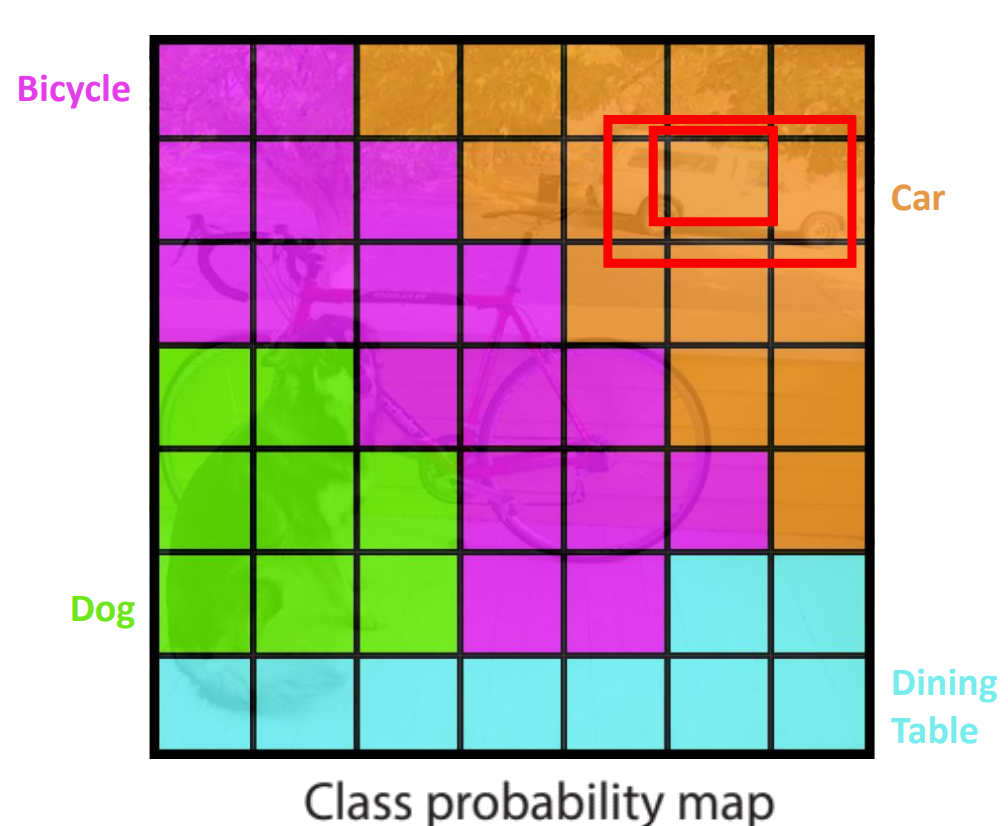
\includegraphics[width=1.0\textwidth,height=1.0\textheight,keepaspectratio]{images/obj-det/yolo_7.png}
    \end{figure}
    }

    \only<6>{
    \begin{figure}
    \centering
    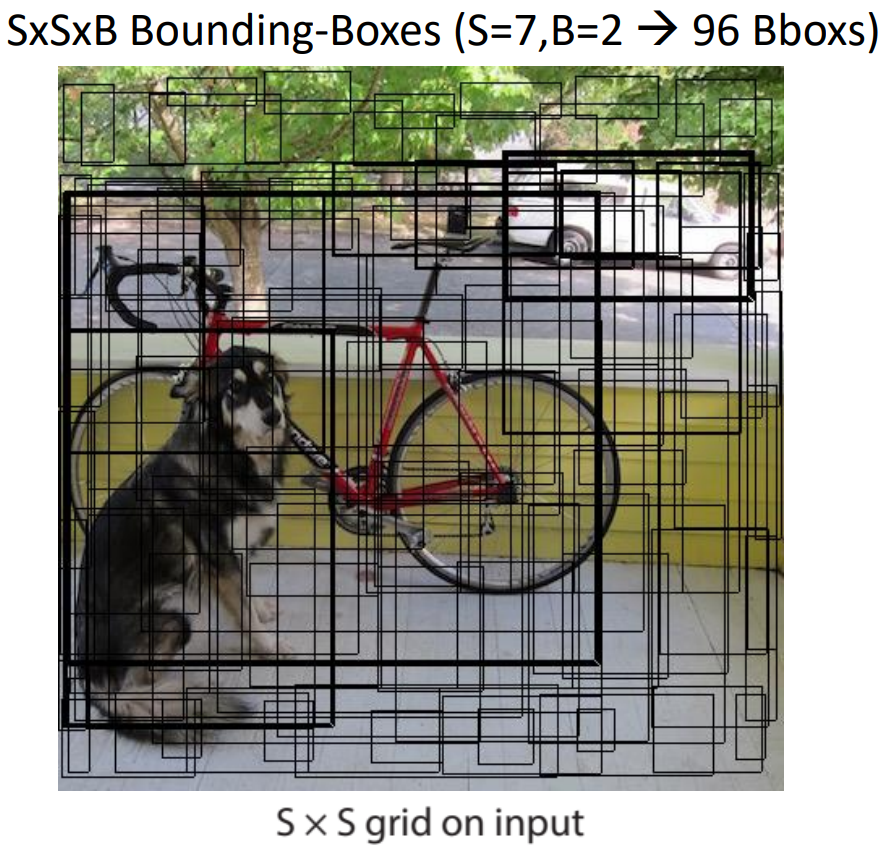
\includegraphics[width=1.0\textwidth,height=1.0\textheight,keepaspectratio]{images/obj-det/yolo_8.png}
    \end{figure}
    }

    \only<7>{
    \begin{figure}
    \centering
    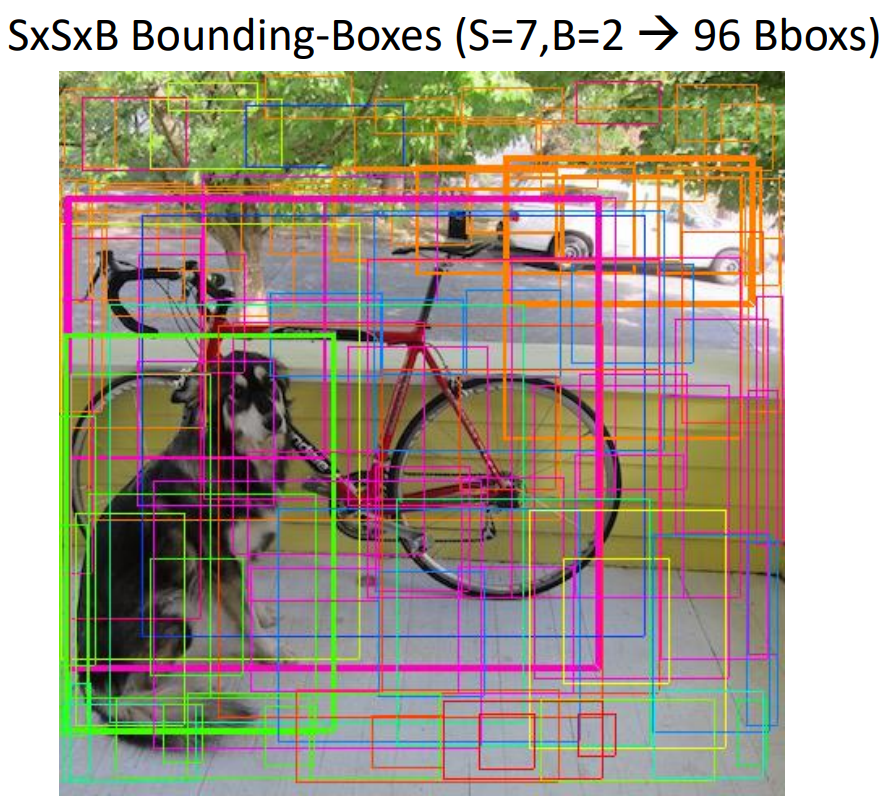
\includegraphics[width=1.0\textwidth,height=1.0\textheight,keepaspectratio]{images/obj-det/yolo_9.png}
    \end{figure}
    }

    \only<8>{
    \begin{figure}
    \centering
    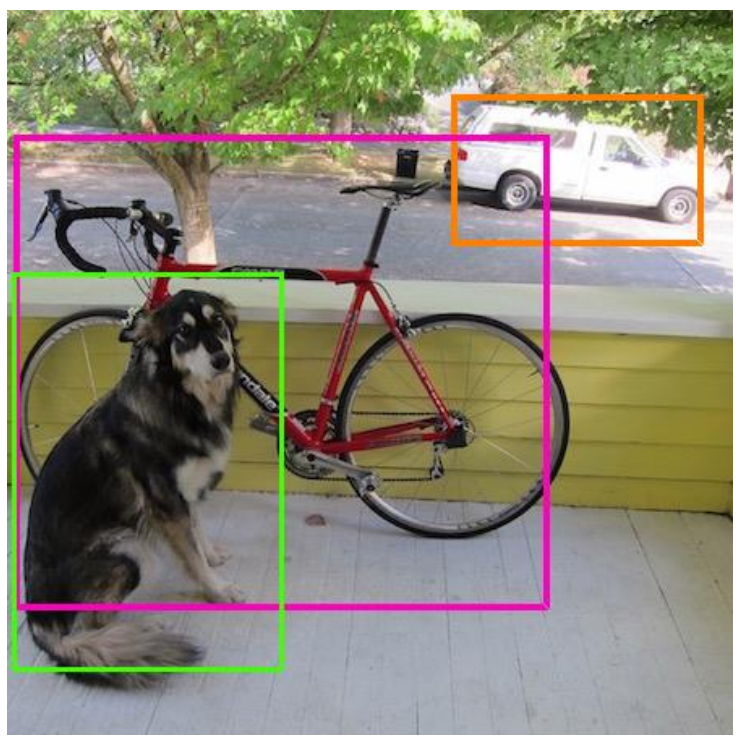
\includegraphics[width=1.0\textwidth,height=1.0\textheight,keepaspectratio]{images/obj-det/yolo_10.png}
    \end{figure}
    }
        
    \end{column}
\end{columns}
    
\end{frame}

\begin{frame}{YOLO - Loss Function}
    \begin{figure}
    \centering
    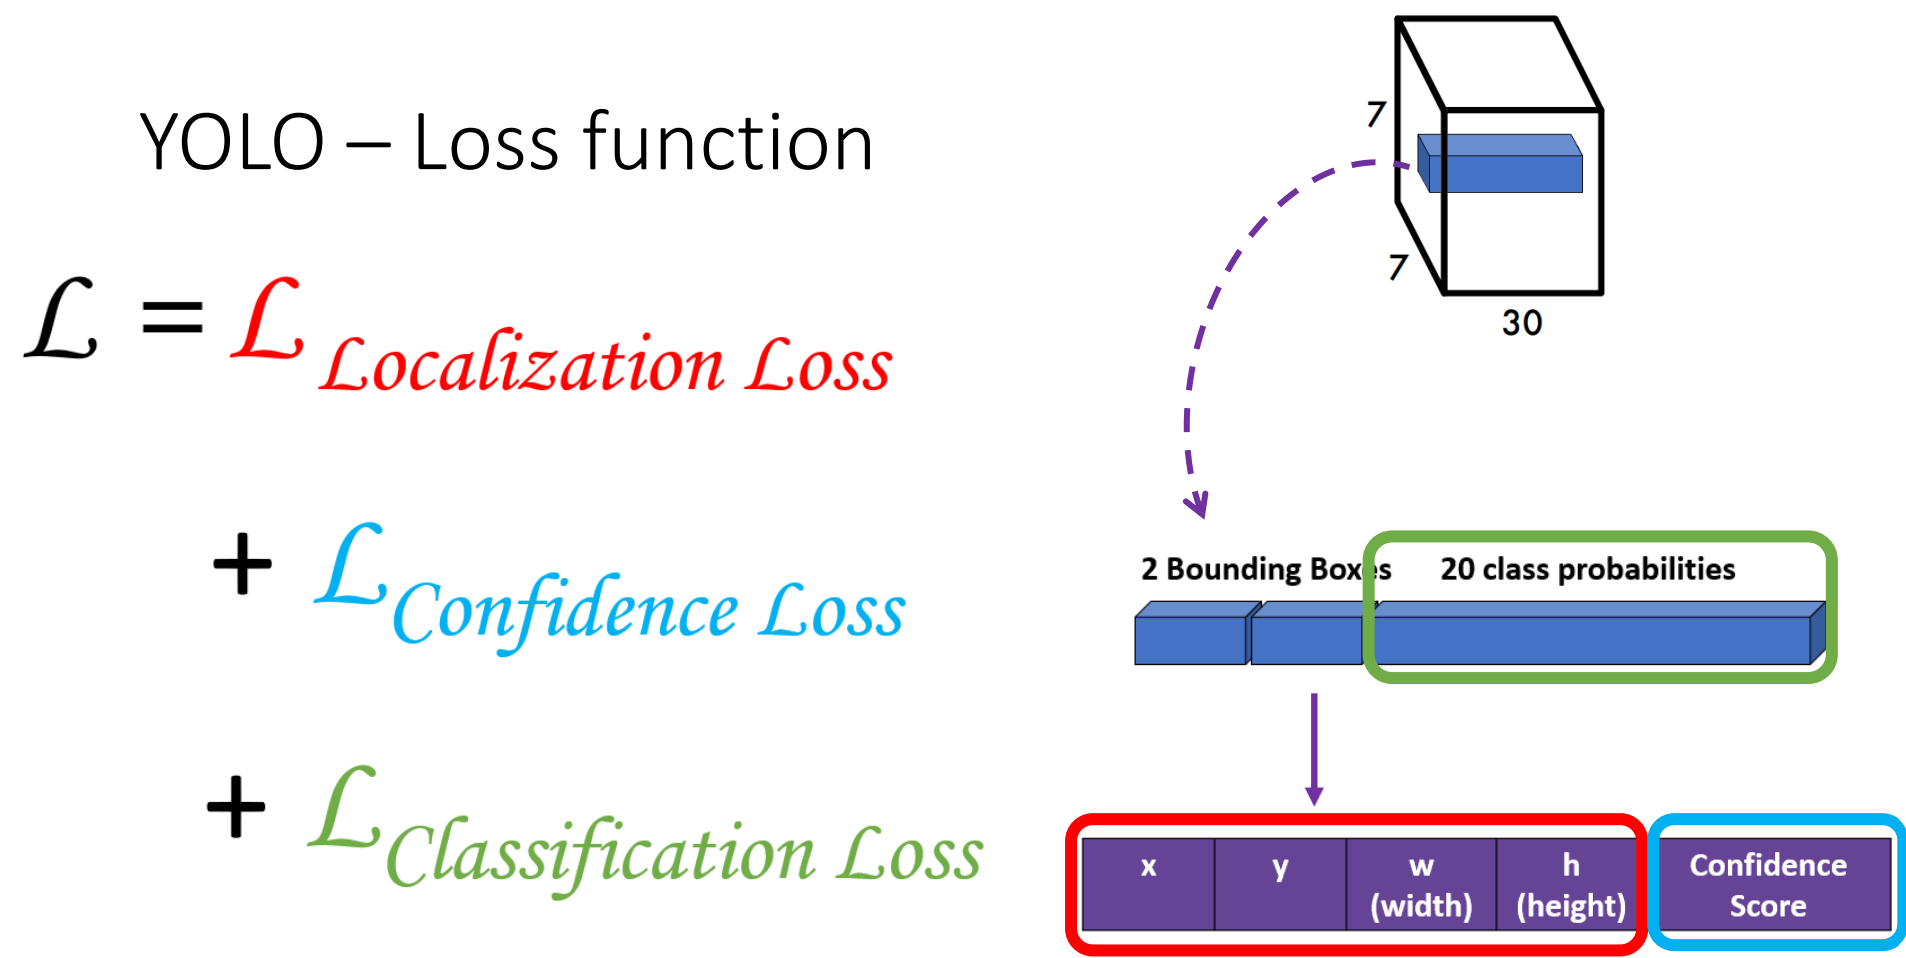
\includegraphics[width=1.0\textwidth,height=1.0\textheight,keepaspectratio]{images/obj-det/yolo_11.png}
    \end{figure}
\end{frame}



\begin{frame}{YOLO - Benefits}
\begin{columns}
    \begin{column}{0.6\textwidth}
    \begin{itemize}
        \item Fast. Good for real-time processing
        \item End-to-end training
    \end{itemize}
    \begin{figure}
    \centering
    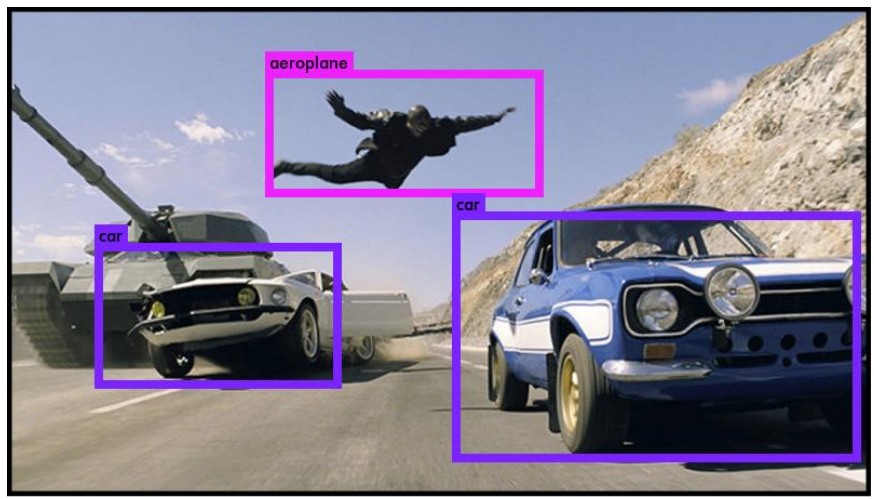
\includegraphics[width=1.0\textwidth,height=1.0\textheight,keepaspectratio]{images/obj-det/yolo_12.png}
    \end{figure}
    
    \end{column}
    
    \begin{column}{0.4\textwidth}
    \begin{figure}
    \centering
    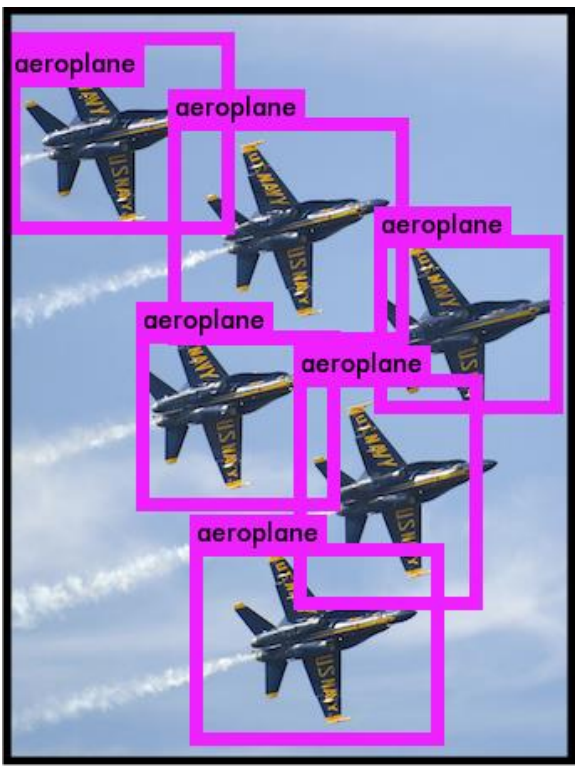
\includegraphics[width=1.0\textwidth,height=0.95\textheight,keepaspectratio]{images/obj-det/yolo_13.png}
    \end{figure}
        
    \end{column}
\end{columns}
    
\end{frame}

\begin{frame}{YOLO - Limitations}
\begin{columns}
    \begin{column}{0.5\textwidth}
    \begin{itemize}
        \item<2-> Difficult to detect small objects
        \item<2-> Coarse predictions
        \item<3-> Fixed input size
        \item<4-> A grid cell can predict only one class
        \vspace{0.5cm}
        \onslide<5->{
        \item \textcolor{red}{Solutions:}
        \begin{itemize}
            \item Remove fc layers!
            \item Predict class per bbox (not per cell)
        \end{itemize}
        }
    \end{itemize}
    \end{column}
    
    \begin{column}{0.5\textwidth}
    \only<-2>{
    \begin{figure}
    \centering
    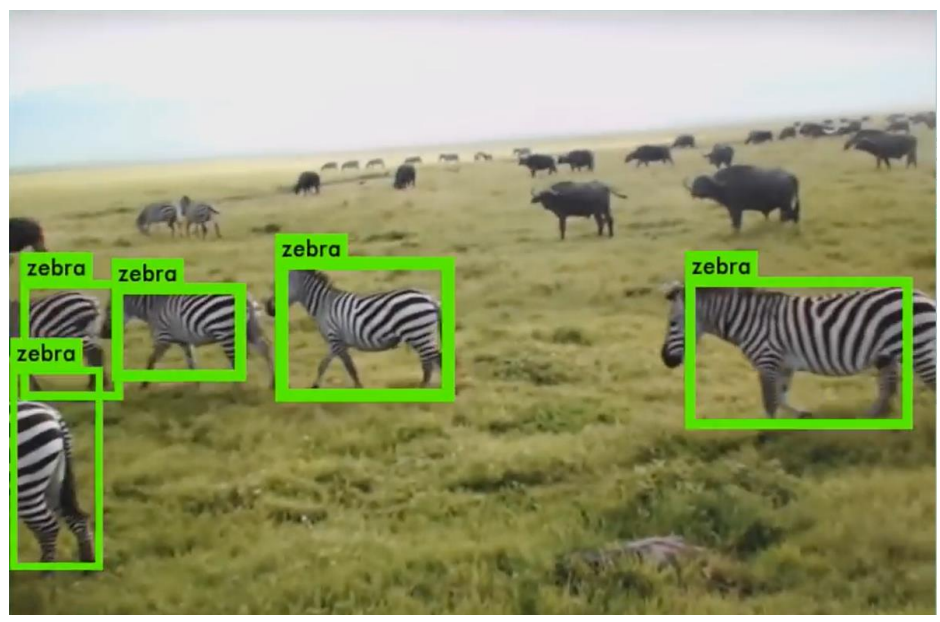
\includegraphics[width=1.0\textwidth,height=1.0\textheight,keepaspectratio]{images/obj-det/yolo_14.png}
    \end{figure}
    }

    \only<3>{
    \begin{figure}
    \centering
    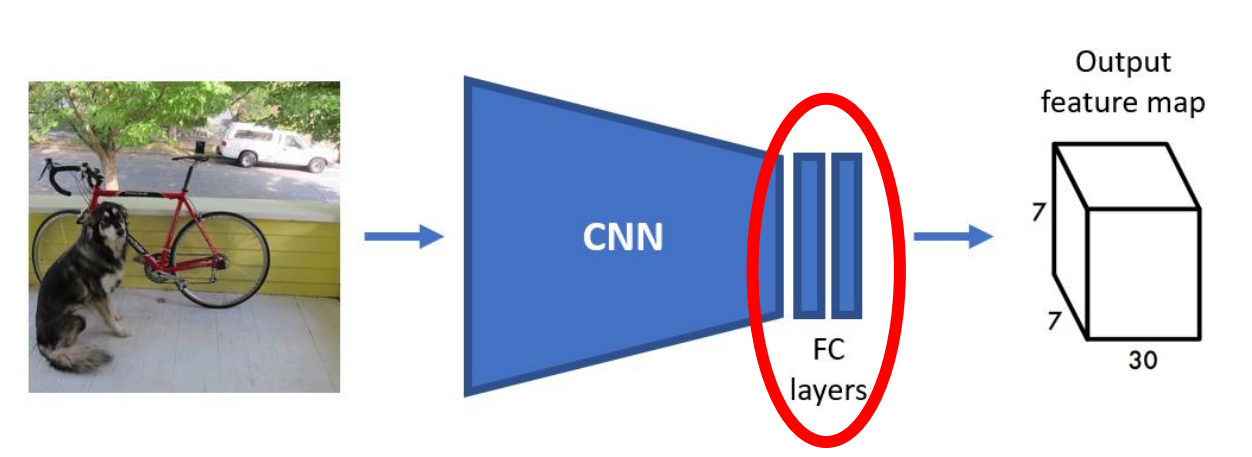
\includegraphics[width=1.0\textwidth,height=1.0\textheight,keepaspectratio]{images/obj-det/yolo_15.png}
    \end{figure}
    }

    \only<4->{
    \begin{figure}
    \centering
    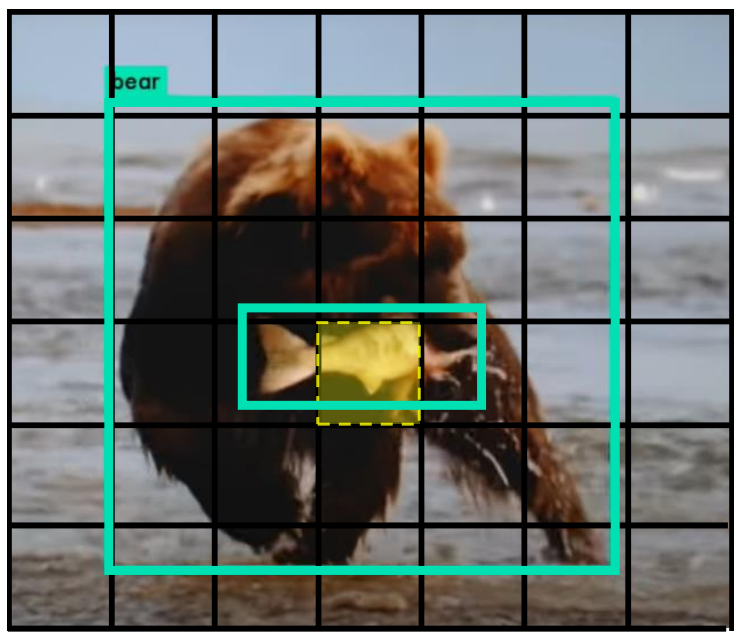
\includegraphics[width=1.0\textwidth,height=1.0\textheight,keepaspectratio]{images/obj-det/yolo_16.png}
    \end{figure}
    }
        
    \end{column}
\end{columns}
\end{frame}

\begin{frame}{YOLOv2}
\begin{itemize}
    \item Removed fully connected layers
    \item A grid cell predicts class probabilities for each box
\end{itemize}
\begin{figure}
\centering
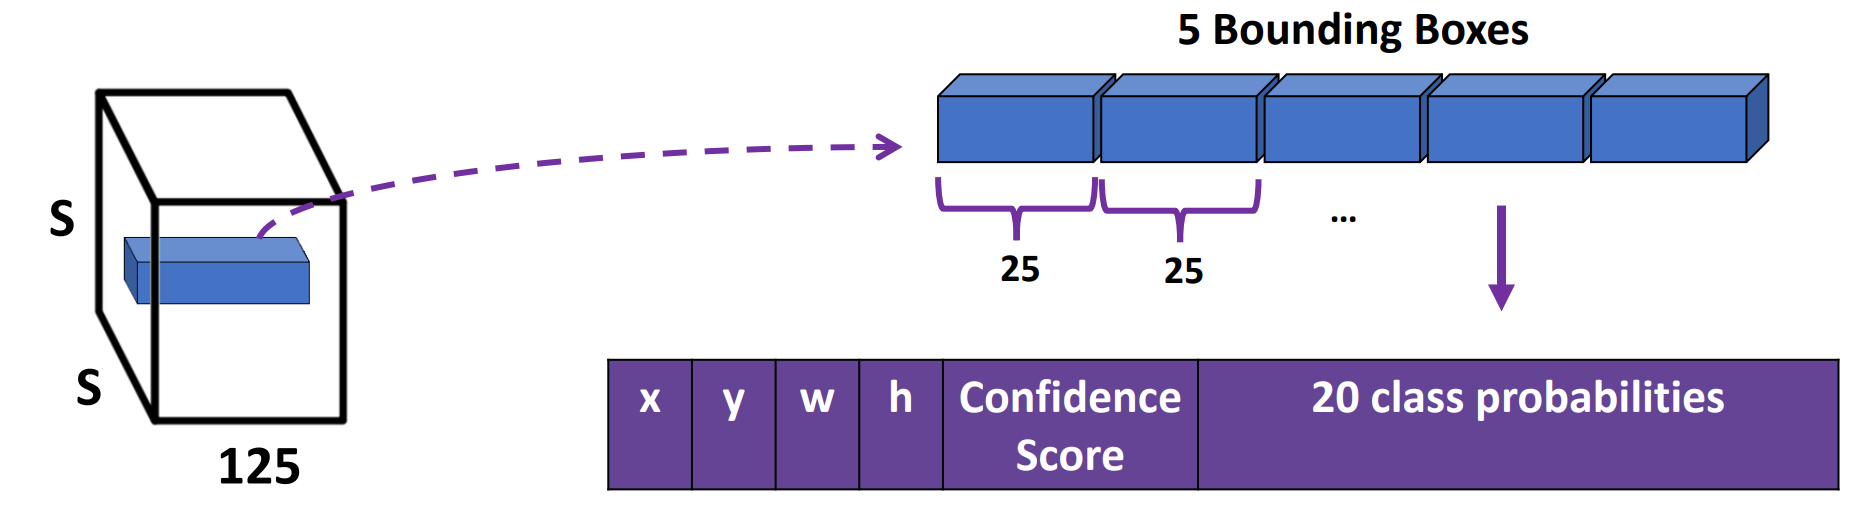
\includegraphics[width=1.0\textwidth,height=1.0\textheight,keepaspectratio]{images/obj-det/yolo_17.png}
\end{figure}

    
\end{frame}

\begin{frame}{There's always room for improvement!}
\begin{itemize}
    \item YOLOv3
    \begin{itemize}
        \item J. Redmon, A. Farhadi. Yolov3: An incremental improvement, 2018
    \end{itemize}
    \item YOLOv4
    \begin{itemize}
        \item A. Bochkovskiy, C. Wang, H. Liao. Yolov4: Optimal speed and accuracy of object detection (Feb. 2020)
    \end{itemize}
    \item YOLOv5
    \begin{itemize}
        \item YOLOv5 by ultralytics (June 2020)
    \end{itemize}
    \item PP-YOLO
    \begin{itemize}
        \item X. Long, K. Deng, G. Wang, Y. Zhang, Q. Dang, Y. Gao, H. Shen, J. Ren, S. Han, E. Ding, S. Wen. Pp-yolo: An effective and efficient implementation of object detector (June 2020)
    \end{itemize}
    \item PP-YOLOv2 (2021)
    \begin{itemize}
        \item J. X. Huang, X. Wang, W. Lv, X. Bai, X. Long, K. Deng, Q. Dang, S. Han, Q. Liu, X. Hu, D. Yu, Y. Ma, O. Yoshie. PP-YOLOv2: A Practical Object Detector (2021)
    \end{itemize}

\end{itemize}
    
\end{frame}